\documentclass[a4paper,12pt]{article} % тип документа
\usepackage[margin=1in]{geometry} % Поля

%  Русский язык
\usepackage[warn]{mathtext}
\usepackage[T2A]{fontenc}			% кодировка
\usepackage[utf8]{inputenc}			% кодировка исходного текста
\usepackage[english,russian]{babel}	% локализация и переносы
% Математика
\usepackage{amsmath,amsfonts,amssymb,amsthm,mathtools} 
\usepackage{wasysym}
%%%
\usepackage{graphicx}

\usepackage{tabularx}

\usepackage{gensymb} % знак градуса
\usepackage{enumitem} % изменить список enumerate
\usepackage{placeins} % \FloatBarrier

\renewcommand{\thesection}{\Roman{section}} 
\renewcommand{\thesubsection}{\roman{subsection}}


\begin{document}

\newcolumntype{Y}{>{\centering\arraybackslash}X} %new tabularx


%титул
\hrule 	
\medskip
\begin{raggedright}
{\large \textbf{Отчёт по работе 3.2.8}}
\\
\medskip
{\Large Релаксационные колебания} 
\\
\medskip
{\large Карташов Констанин Б04-005}
\medskip
\hrule
\medskip
\end{raggedright}


\section{Анотация}

\paragraph{Цель работы:} 
Изучение вольт-амперной характеристики нормального
тлеющего разряда; исследование релаксационного генератора на стабилитроне.

\paragraph{Оборудование:}
\begin{itemize}
\renewcommand{\labelitemi}{$\triangleright$}
\itemsep0em
\item Стабилитрон СГ-2
\item Амперметр
\item Вольтметр 
\item Магазин сопротивлений
\item Магазин ёмкостей
\item Источник питания
\item Осциллограф
\item Генератор звуковой частоты
\end{itemize}


\medskip\hrule\medskip

\section{Теоретическая часть}

\subsection{Некоторые сведения}

Релаксационные колебания -- это такие колебания, в которых происходит зарядка и разрядка всего одного накопителя энергии. В нашем случае накопителем энергии является конденсатора, а режим зарядки и разрядки регулируется газоразрядным диодом -- стабилитроном. Стабилитрон нелинейный элемент, пропускающий ток при достижении потенциала зажигания $V_1$, и перестающий пропускать его при достижения потенциала затухания $V_2 < V_1$, за счёт чего обеспечиваются колебания. Период колебания такой схемы определяется временем зарядки конденсатора.

Напряжение на кондесаторе, когда выключен стабилитрон:

\[ RC \frac{dV}{dt} = U - V, \]

проинтегрировав, и подставив начальное напряжения $V_1$, конечное $V_2$ и время $\tau_\text{заж}$:

\[ V_1 = U - (U - V_2) e ^ {\tau_\text{заж}/RC}, \]

\[T \approx \tau_\text{зат} = RC \ln \left( \frac{U - V_2}{U - V_1} \right).\]

\begin{figure}
\begin{center}
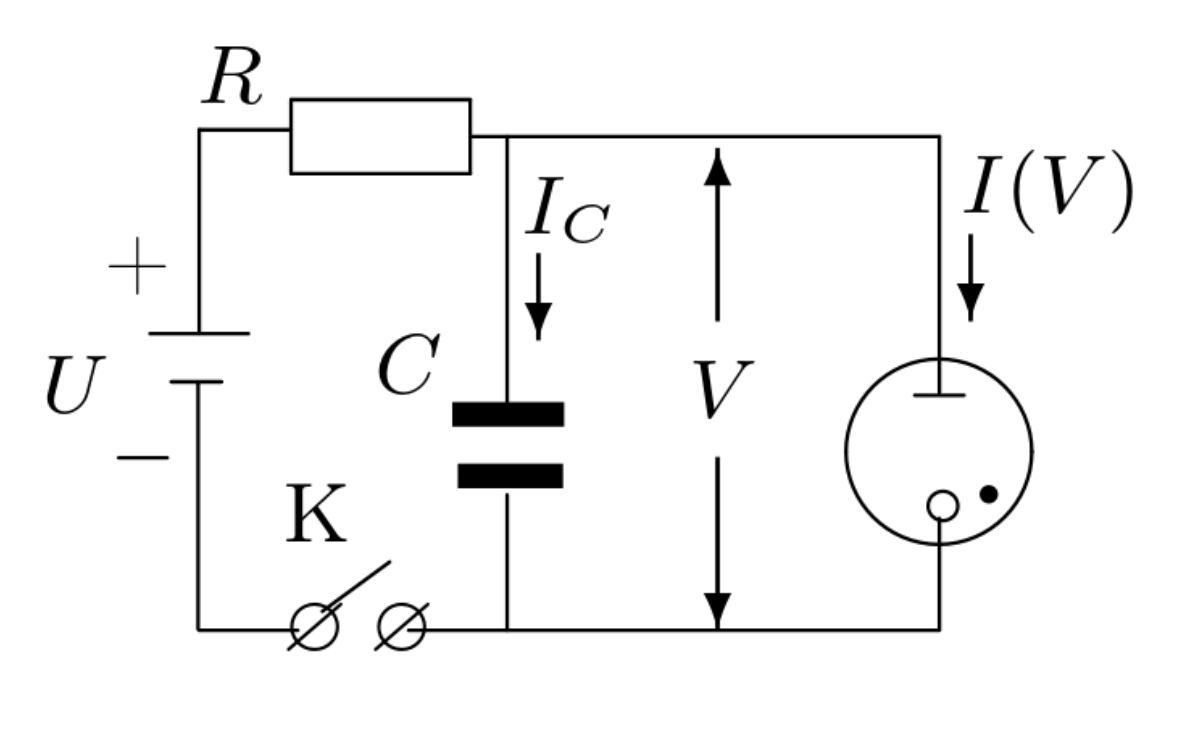
\includegraphics[width=0.5\textwidth]{scheme1.png}
\caption{Принципиальная схема релаксационного генератора}
\label{fig:sc1}
\end{center}
\end{figure}


\medskip\hrule\medskip

\section{Экспериментальная часть}

\subsection{Измерение ВАХ стабилитрона}

\begin{figure}
\begin{center}
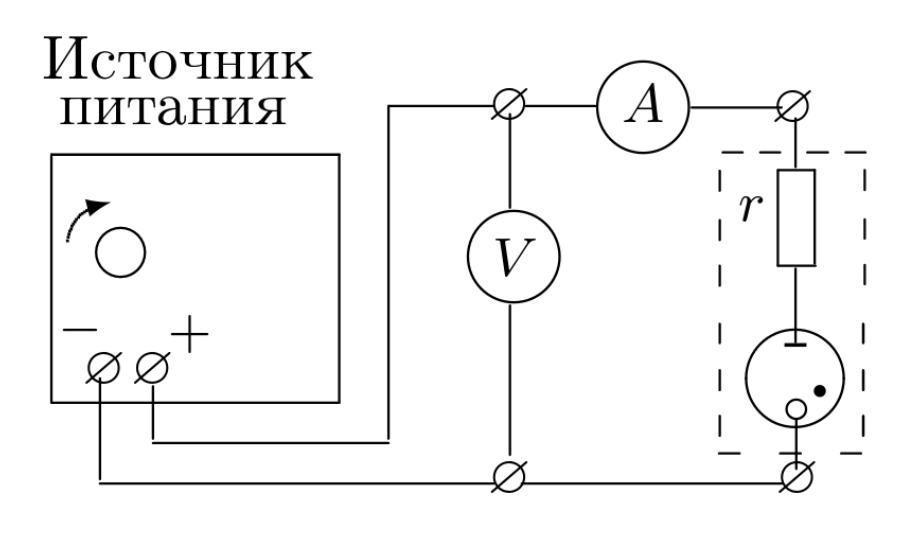
\includegraphics[width=0.5\textwidth]{scheme2.png}
\caption{Схема установки для изучения характеристик стабилитрона}
\label{fig:sc2}
\end{center}
\end{figure}

\paragraph{} Соберём установку для снятия ВАХ (рис. \ref{fig:sc2}). В первую очередь определим потенциалы зажигания и гашения. Для этого постепенно будем повышать напряжение, до зажигания диода, напряжение при котором диод зароится будет потенциалом загорания $V_1$. Проведём те же самые действия, но при уменьшении напряжения и найдём потенциал гашения. Получаем:

\[ V_1 = 96 \; \text{В}, \;\;\; V_2 = 76 \text{В} .\]

\paragraph{} Теперь снимем ВАХ для зажжённого стабилитрона. Будем снимать значения тока сначала повышая напряжение, а затем его понижая. Результаты занесём в таблицу, и по ним построим график.

\begin{table}[h]
\begin{center}
\begin{tabularx}{\textwidth}{|Y||X|X|X|X|X|X|X|}
\hline 
$U$, В & 88.8 & 96.5 & 105.6 & 107.5 & 115.2 & 110.2 & 100.4 \\ 
\hline 
$I$, мА & 2.9 & 4.2 & 5.9 & 6.3 & 7.7 & 6.8 & 5.1 \\ 
\hline 
$U$, В & 95.7 & 90.8 & 88.8 & 84.2 & 82.9 & 78.6 & 76.8 \\ 
\hline 
$I$, мА & 4.2 & 3.3 & 2.9 & 2.1 & 1.9 & 1.1 & 0.8 \\ 
\hline 
\end{tabularx}
\label{tab1}
\caption{Значения снятые для построения ВАХ стабилитрона} 
\end{center}
\end{table}

\begin{figure}
\begin{center}
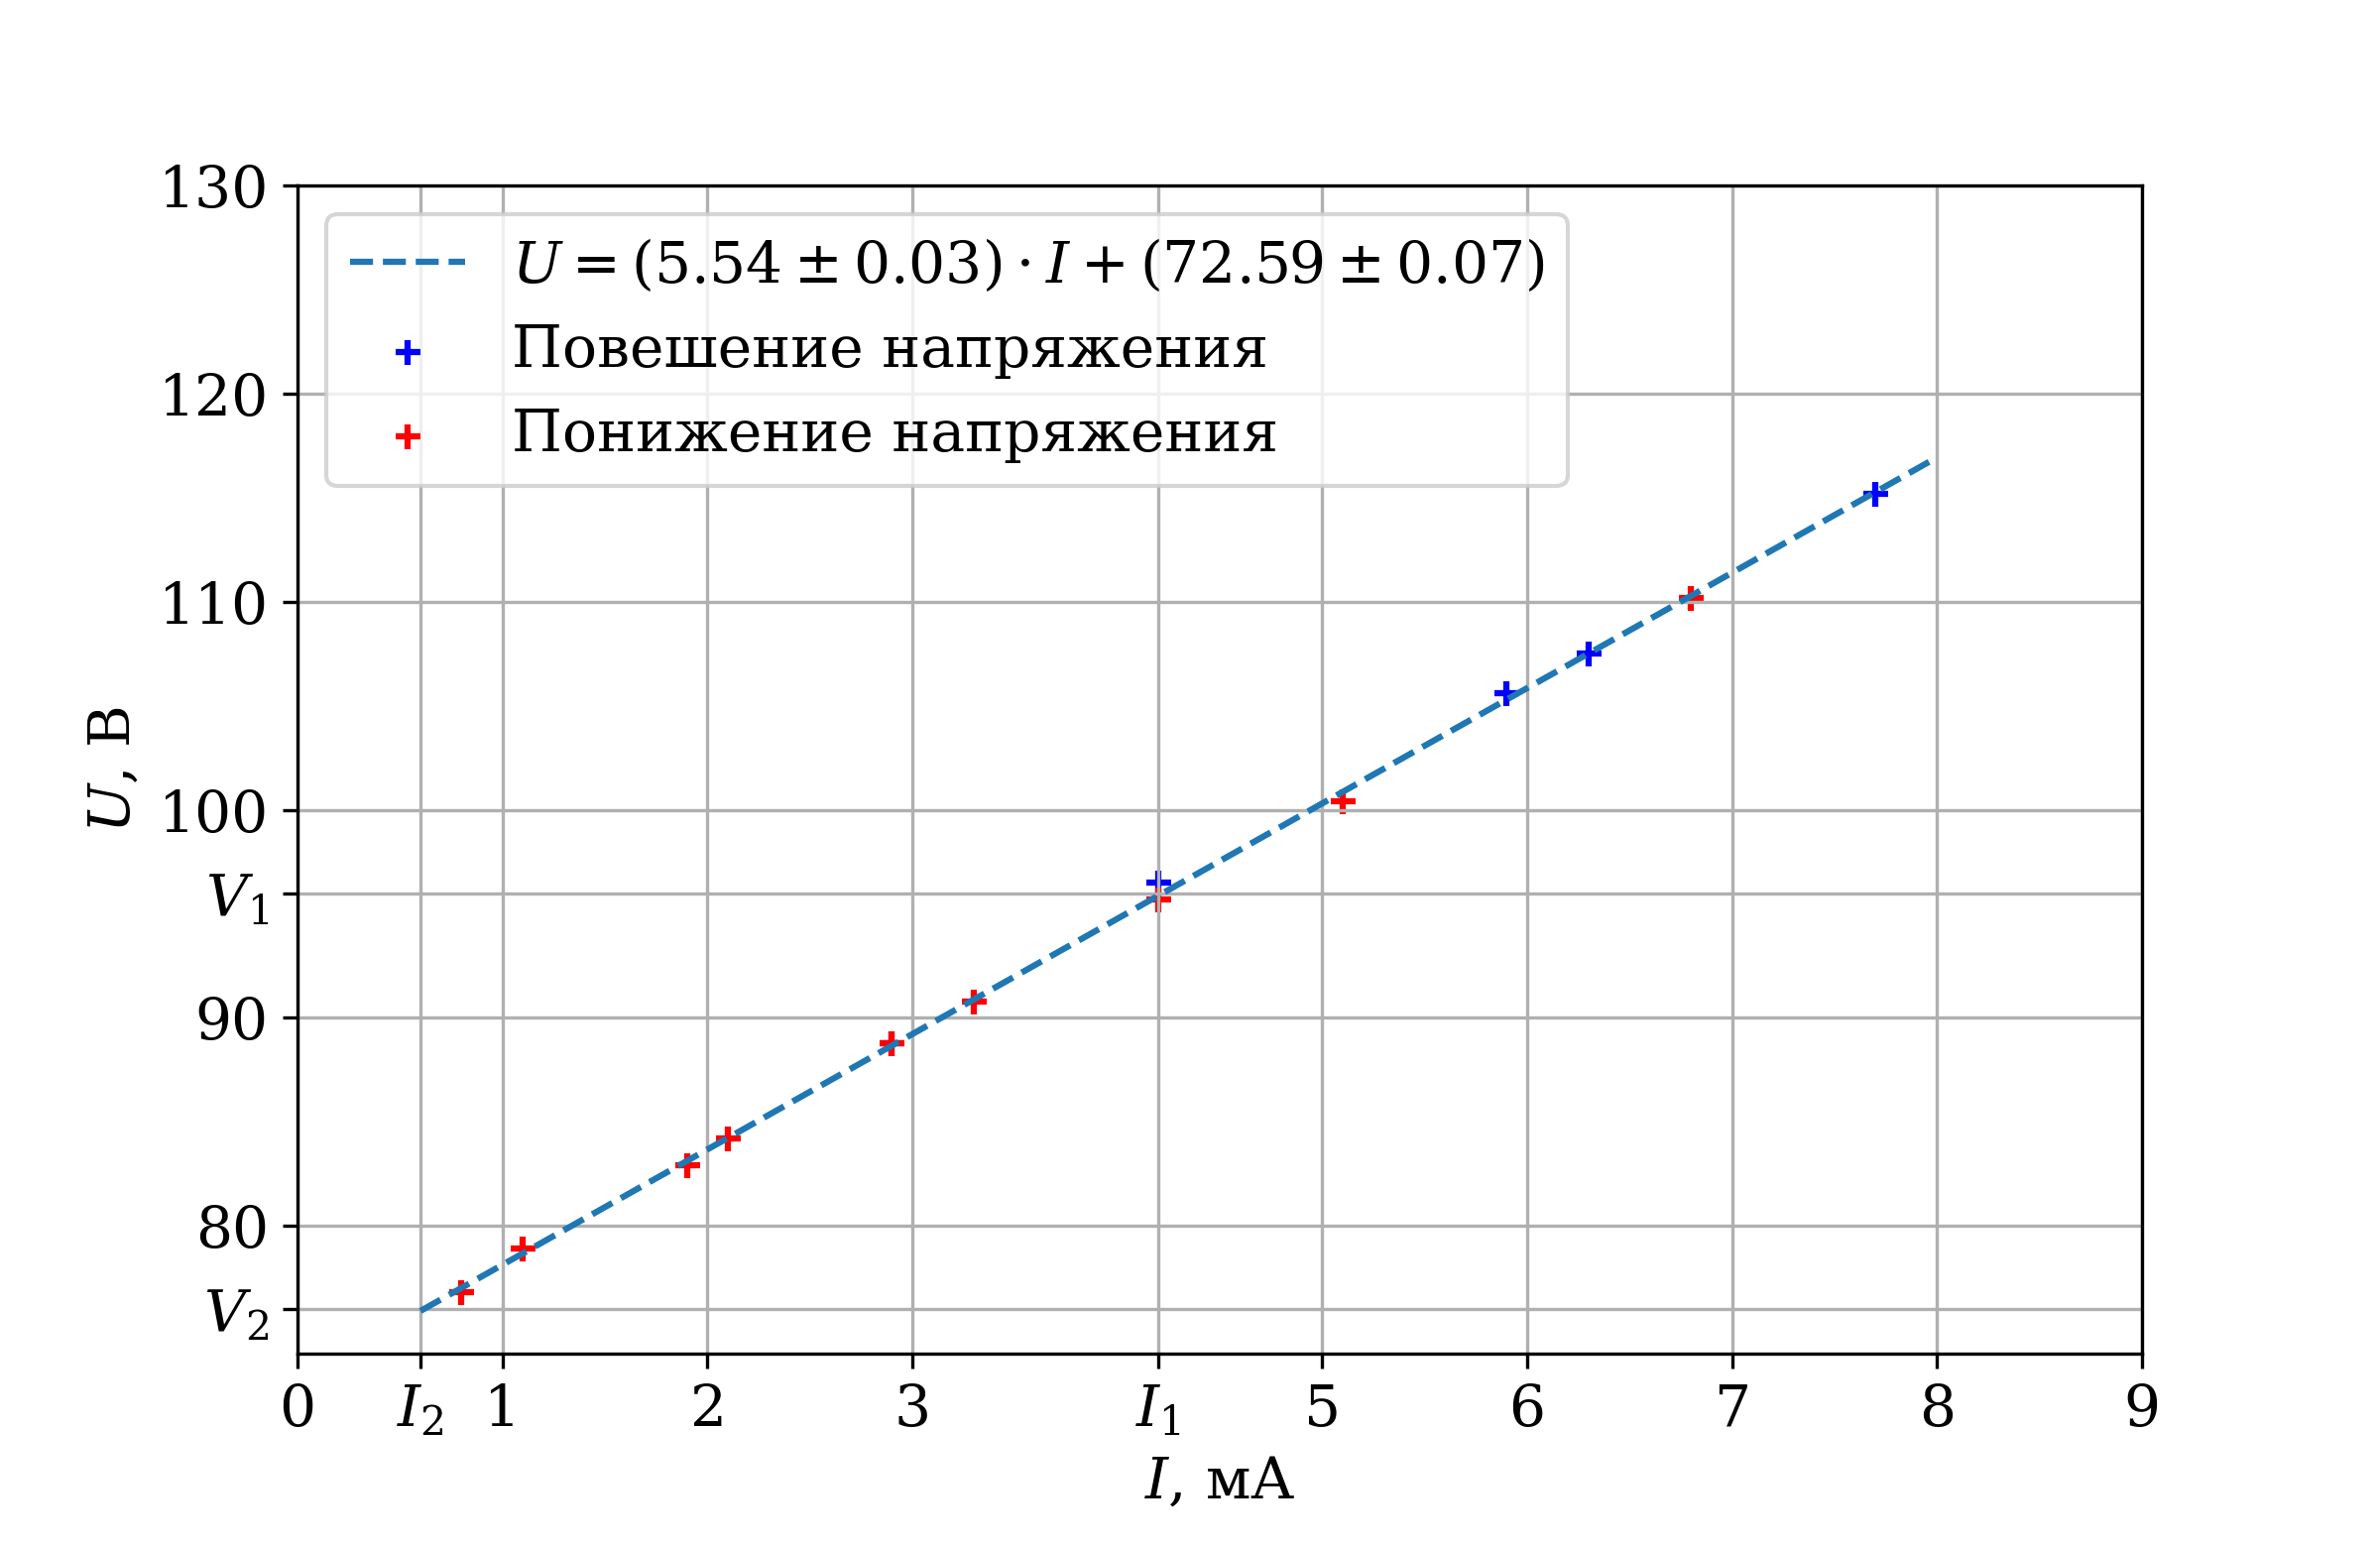
\includegraphics[width=1\textwidth]{plot1.png}
\caption{График измеренной ВАХ стабилитрона}
\label{fig:1}
\end{center}
\end{figure}

\paragraph{} По графику видим, что все точки лежат на прямой, как и должно быть в теории. Аппроксимирующую прямую посчитаем пользуясь методом наименьших квадратов. И изобразим её на графике.
Точку не лежащую на прямой ($I = 5.5$ мА, $U = 10$) из расчётов исключим. 


По полученной прямой рассчитаем значения для тока зажигания и потухания. Из чего получим:

\[ I_1 = 4.2 \; \text{мА},\;\;\; I_2 = 0.6 \; \text{мА}.\]

\subsection{Изучение осциллограммы релаксационных колебаний}

\begin{figure}[h]	
\begin{center}
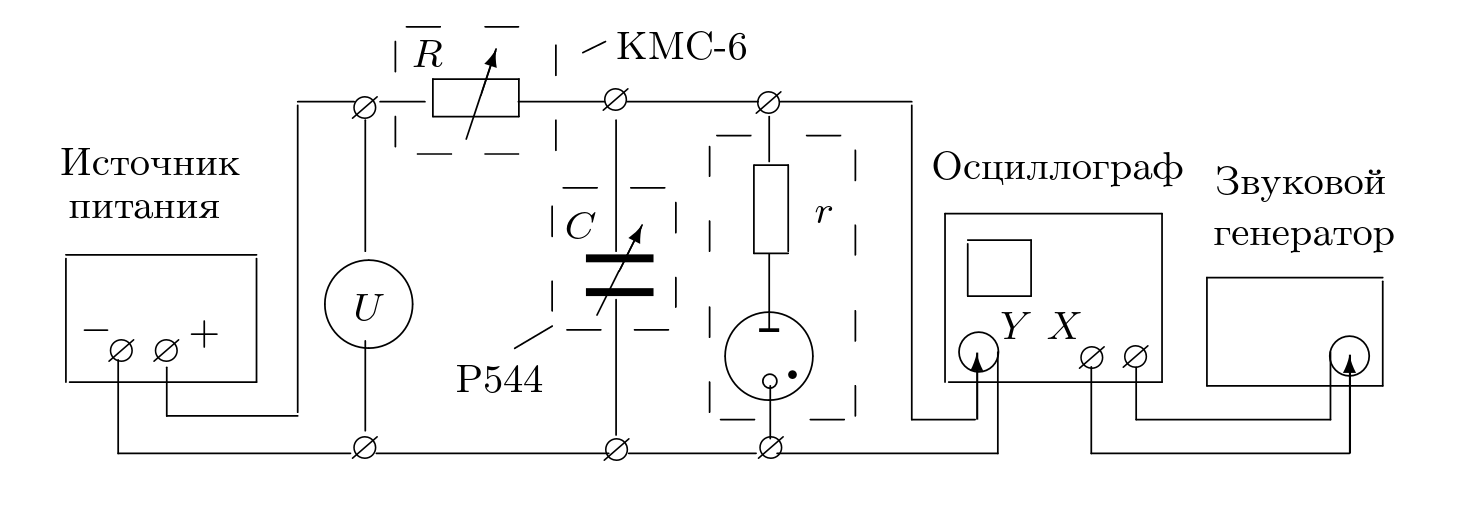
\includegraphics[width=1\textwidth]{scheme3.png}
\caption{Схема установки для исследования релаксационных колебаний.}
\label{fig:sc3}
\end{center}
\end{figure}

\paragraph{} Соберём экспериментальную установку (рис. \ref{fig:sc3}). Выставим значения $R = 900$ кОм, $C = 5 \cdot 10^{-2}$ мкФ. Выставим напряжение $U = 118.5$ В $\approx 1.2 V_1$.

Получим на осциллографе изображение пилообразных колебаний (рис. \ref{fig:saw}). По изображению оценим $\tau_\text{заг}:\tau_\text{пот} = 70:3$, т.е. можно считать, что $\tau_\text{пот} \ll \tau_\text{заг}$.

\begin{figure}
\begin{center}
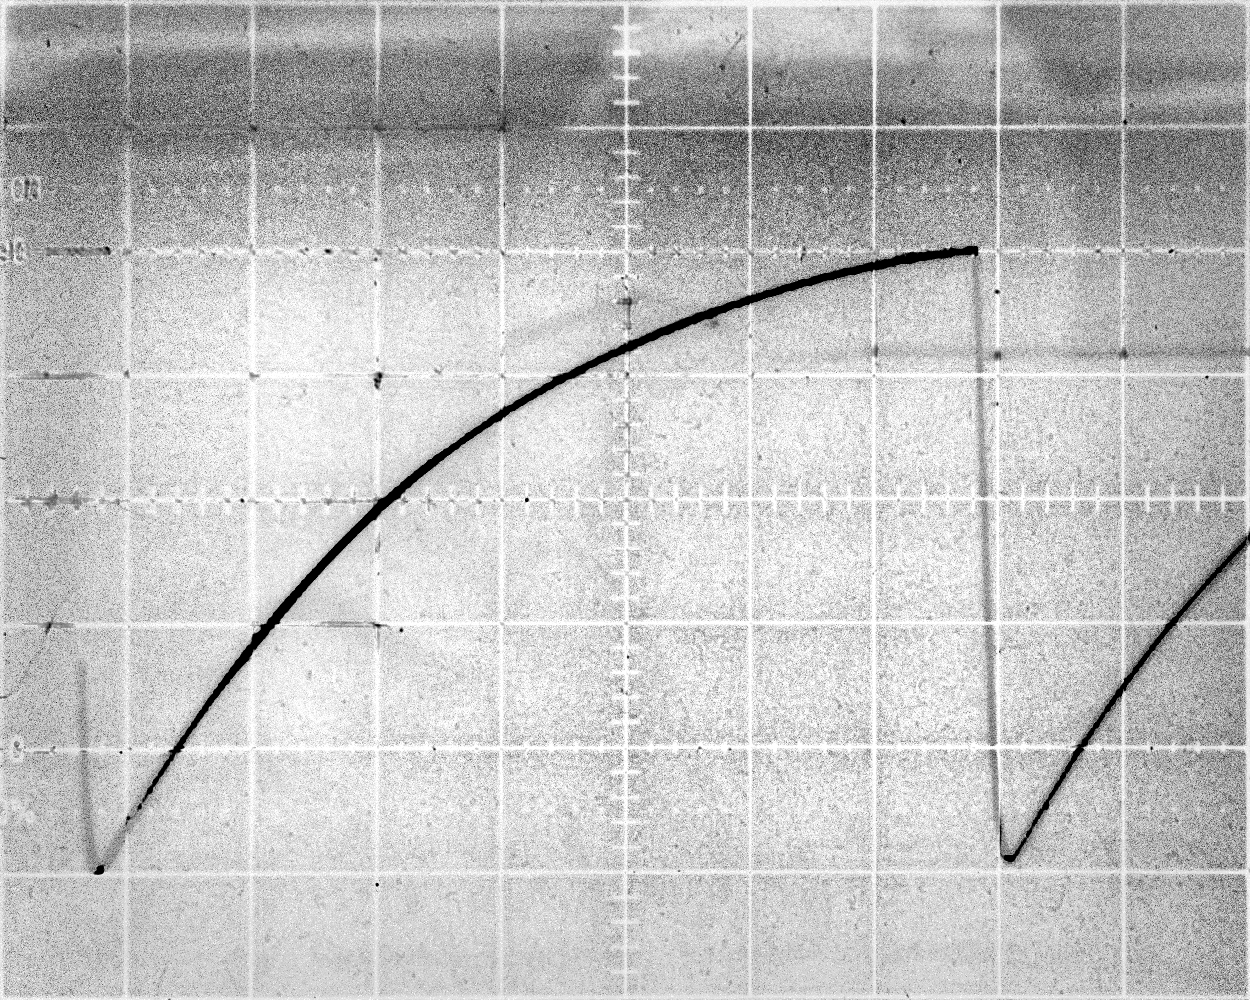
\includegraphics[width=0.7\textwidth]{sawtooth.png}
\caption{Изображение пилообразных колебаний полученных на осциллографе}
\label{fig:saw}
\end{center}
\end{figure}

\paragraph{} Уменьшая сопротивление магазина найдём критическое сопротивление при котором колебания останавливаются. Получим $R_\text{кр} = 120$ кОм. Теоретическое значение для $R_\text{кр} = (U - V_2) / I_2 = (118.5 - 76) / 0.6 = 71$ кОм. Из этого можно сделать заключение, что $V_2$ для динамического значительно случая ниже, чем для статического.

\subsection{Получение фигур Лиссажу и изучение частоты колебаний}

\paragraph{} Восстановим исходные параметры релаксационного генератора. Теперь подадим на вход осциллографа X синусоидальных сигнал с генератора звуковых частот. И пронаблюдаем фигуры Лиссажу для различных отношений частот (рис. \ref{fig:lis11} -- \ref{fig:lis31}).

\begin{figure}[h]
\begin{center}
\begin{minipage}[h]{0.49\textwidth}
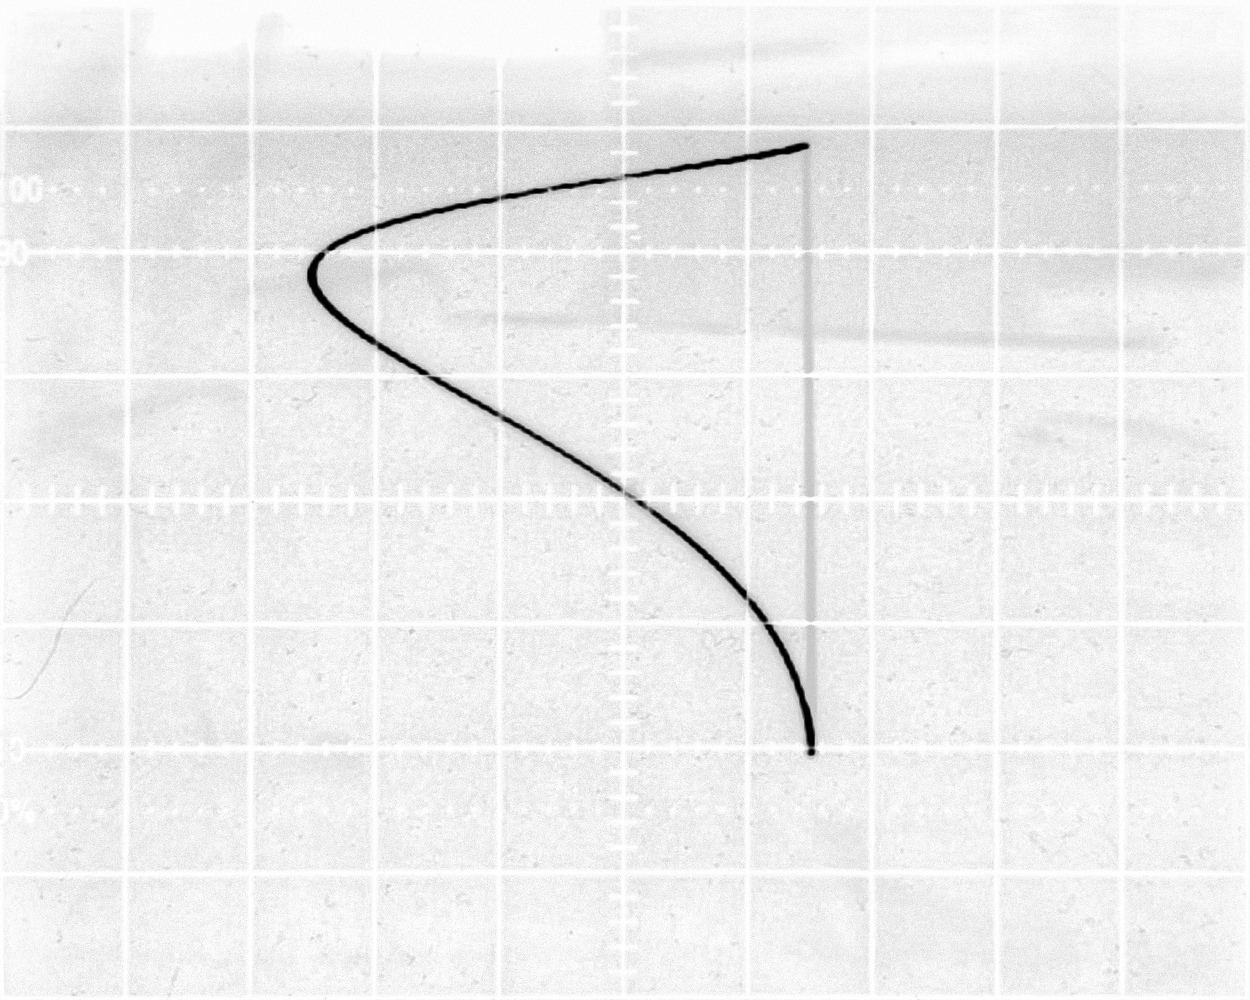
\includegraphics[width=\textwidth]{1-1.jpg}
\caption{Фигура Лиссажу для отношения частот 1:1} 
\label{fig:lis11}
\hfill
\end{minipage}
\begin{minipage}[h]{0.49\textwidth}
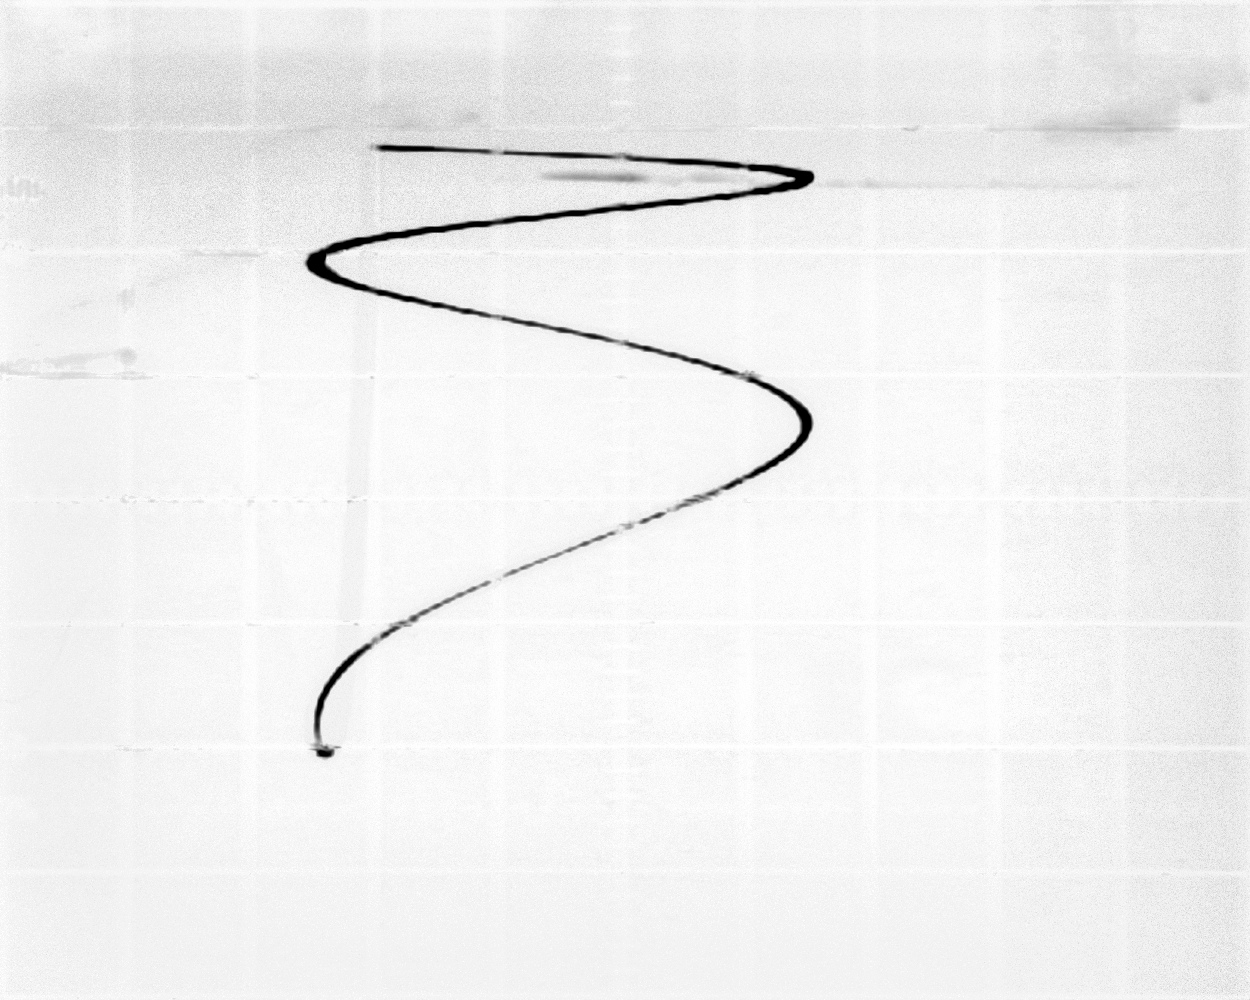
\includegraphics[width=\textwidth]{1-2.jpg}
\caption{Фигура Лиссажу для отношения частот 1:2}
\label{fig:lis12}
\hfill
\end{minipage}

\begin{minipage}[h]{0.49\textwidth}
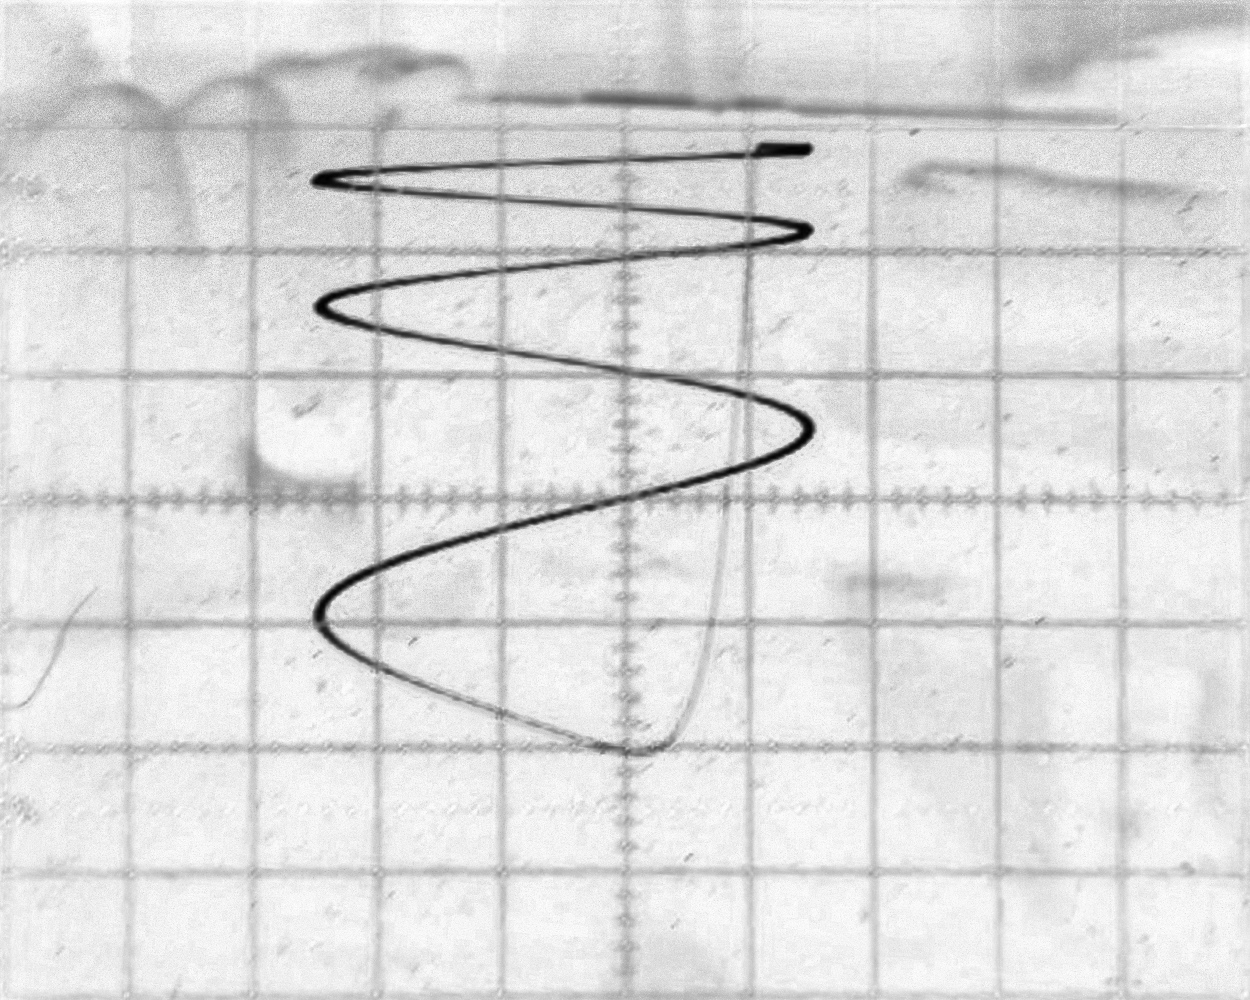
\includegraphics[width=\textwidth]{1-3.jpg}
\caption{Фигура Лиссажу для отношения частот 1:3} 
\label{fig:lis13}
\hfill
\end{minipage}
\begin{minipage}[h]{0.49\textwidth}
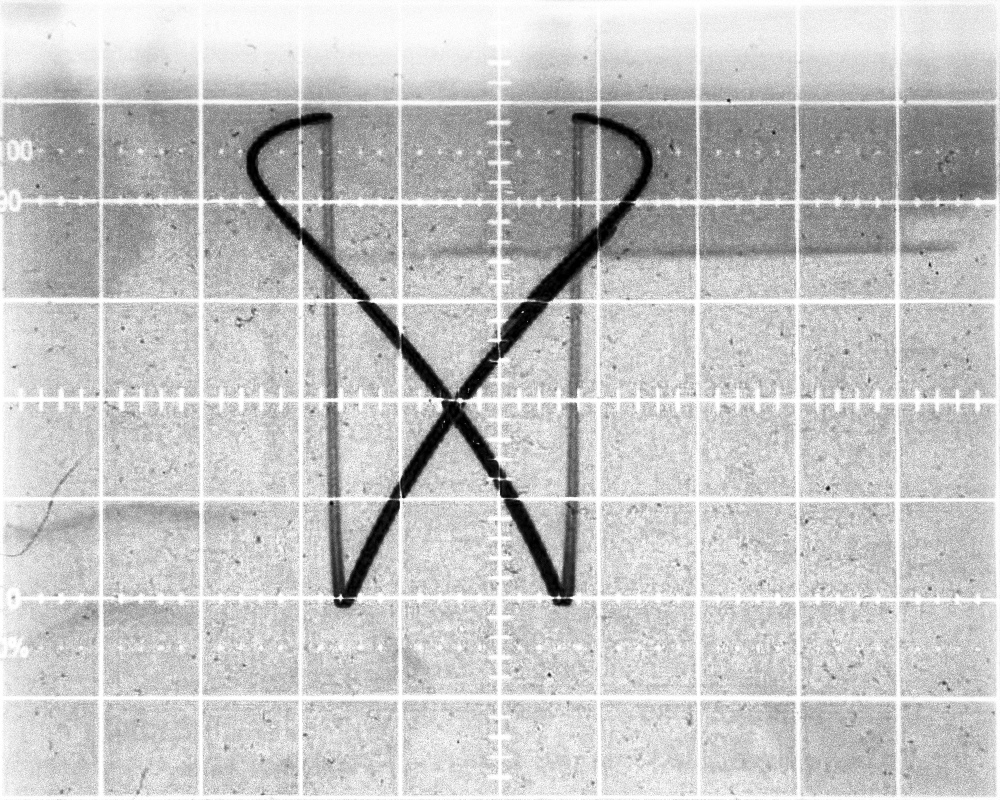
\includegraphics[width=\textwidth]{2-1.jpg}
\caption{Фигура Лиссажу для отношения частот 2:1}
\label{fig:lis21}
\hfill
\end{minipage}

\begin{minipage}[h]{0.49\textwidth}
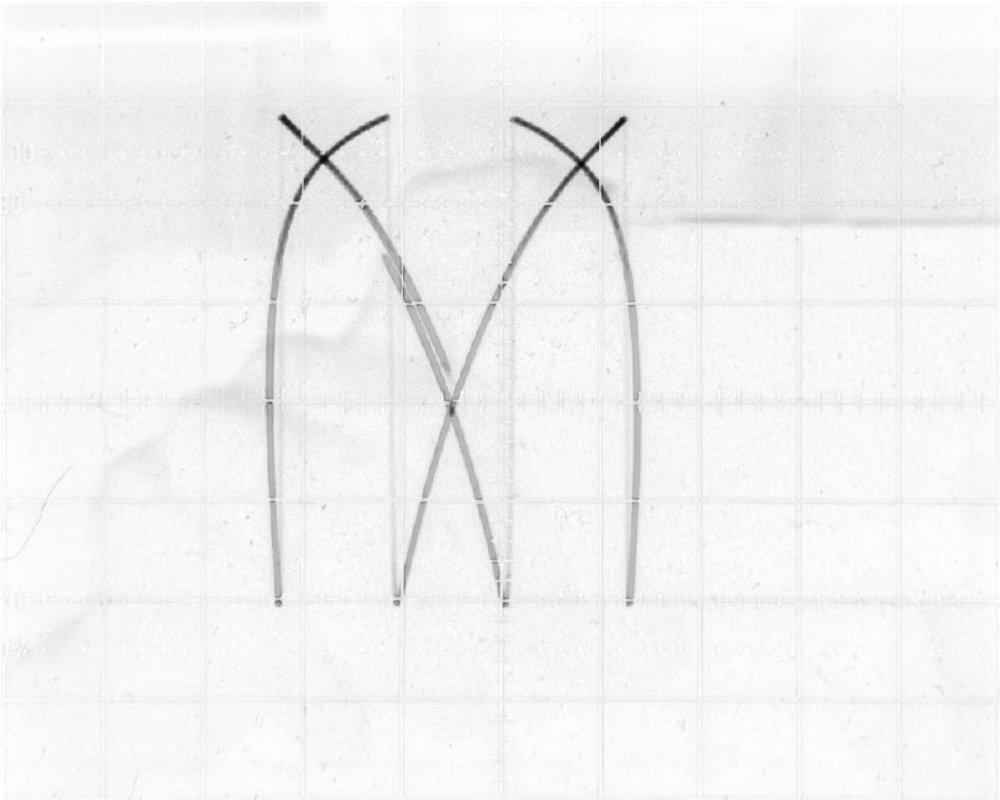
\includegraphics[width=\textwidth]{3-1.jpg}
\caption{Фигура Лиссажу для отношения частот 3:1}
\label{fig:lis31}
\end{minipage}
\end{center}
\end{figure}

\paragraph{} Теперь измерим зависимость частоты колебаний от ёмкости конденсатора при постоянном сопротивлении, и зависимость частоты от сопротивления при постоянной ёмкости. Для измерения частоты будем подбирать частоту генератора звуковых сигналов так, чтобы получались фигуры Лиссажу отношения 1:1.

Измерим $\nu(C)$ при $R = 600$ кОм. Данные занесём в таблицу \ref{tab2}.

\begin{table}[h]
\begin{center}
\begin{tabularx}{\textwidth}{|c||X|X|X|X|X|X|X|X|}
\hline 
$C$, мкФ$\cdot 10^{-3}$ & 50 & 40 & 30 & 20 & 15 & 10 & 8 & 5 \\ 
\hline 
$\nu$, Гц & 39.6 & 45.8 & 60.4 & 90.2 & 119 & 180 & 226 & 363 \\ 
\hline 
$T$, мс & 25.3 & 21.8 & 16.6 & 11.1 & 8.4 & 5.6 & 4.4 & 2.8 \\ 
\hline 
\end{tabularx} 
\caption{Данные измерения зависимости частоты от ёмкости}
\label{tab2}
\end{center}
\end{table}

Измерим $\nu(R)$ при $C = 5 \cdot 10^{-2}$ мкФ. Данные занесём в таблицу \ref{tab3}.

\begin{table}[h]
\begin{center}
\begin{tabularx}{\textwidth}{|c||X|X|X|X|X|X|X|X|X|}
\hline
$R$, кОм  & 900  & 800  & 700  & 600  & 200  & 400  & 300  & 200   & 130 \\
\hline
$\nu$, Гц & 25.1 & 28.7 & 32.8 & 38.2 & 46.1 & 57.4 & 75.4 & 106.3 & 147 \\
\hline
$T$, мс   & 39.8 & 34.8 & 30.5 & 26.2 & 21.7 & 17.4 & 13.3 & 9.4 & 6.8 \\
\hline
\end{tabularx} 
\caption{Данные измерения зависимости частоты от сопротивления}
\label{tab3}
\end{center}
\end{table}

\paragraph{} Теоретическая зависимость определяется по формуле:

\[T \approx \tau_\text{зат} = RC \ln \left( \frac{U - V_2}{U - V_1} \right).\]

На графиках построим точки из табл. \ref{tab2} и \ref{tab3}, и теоретическую зависимость.  Видим, что наклон теоретического и действительного графика сильно отличаются. По наклону графика найдём действительное значения для $V_2$, считая, что $V_1$ постоянно.

\begin{figure}
\begin{center}
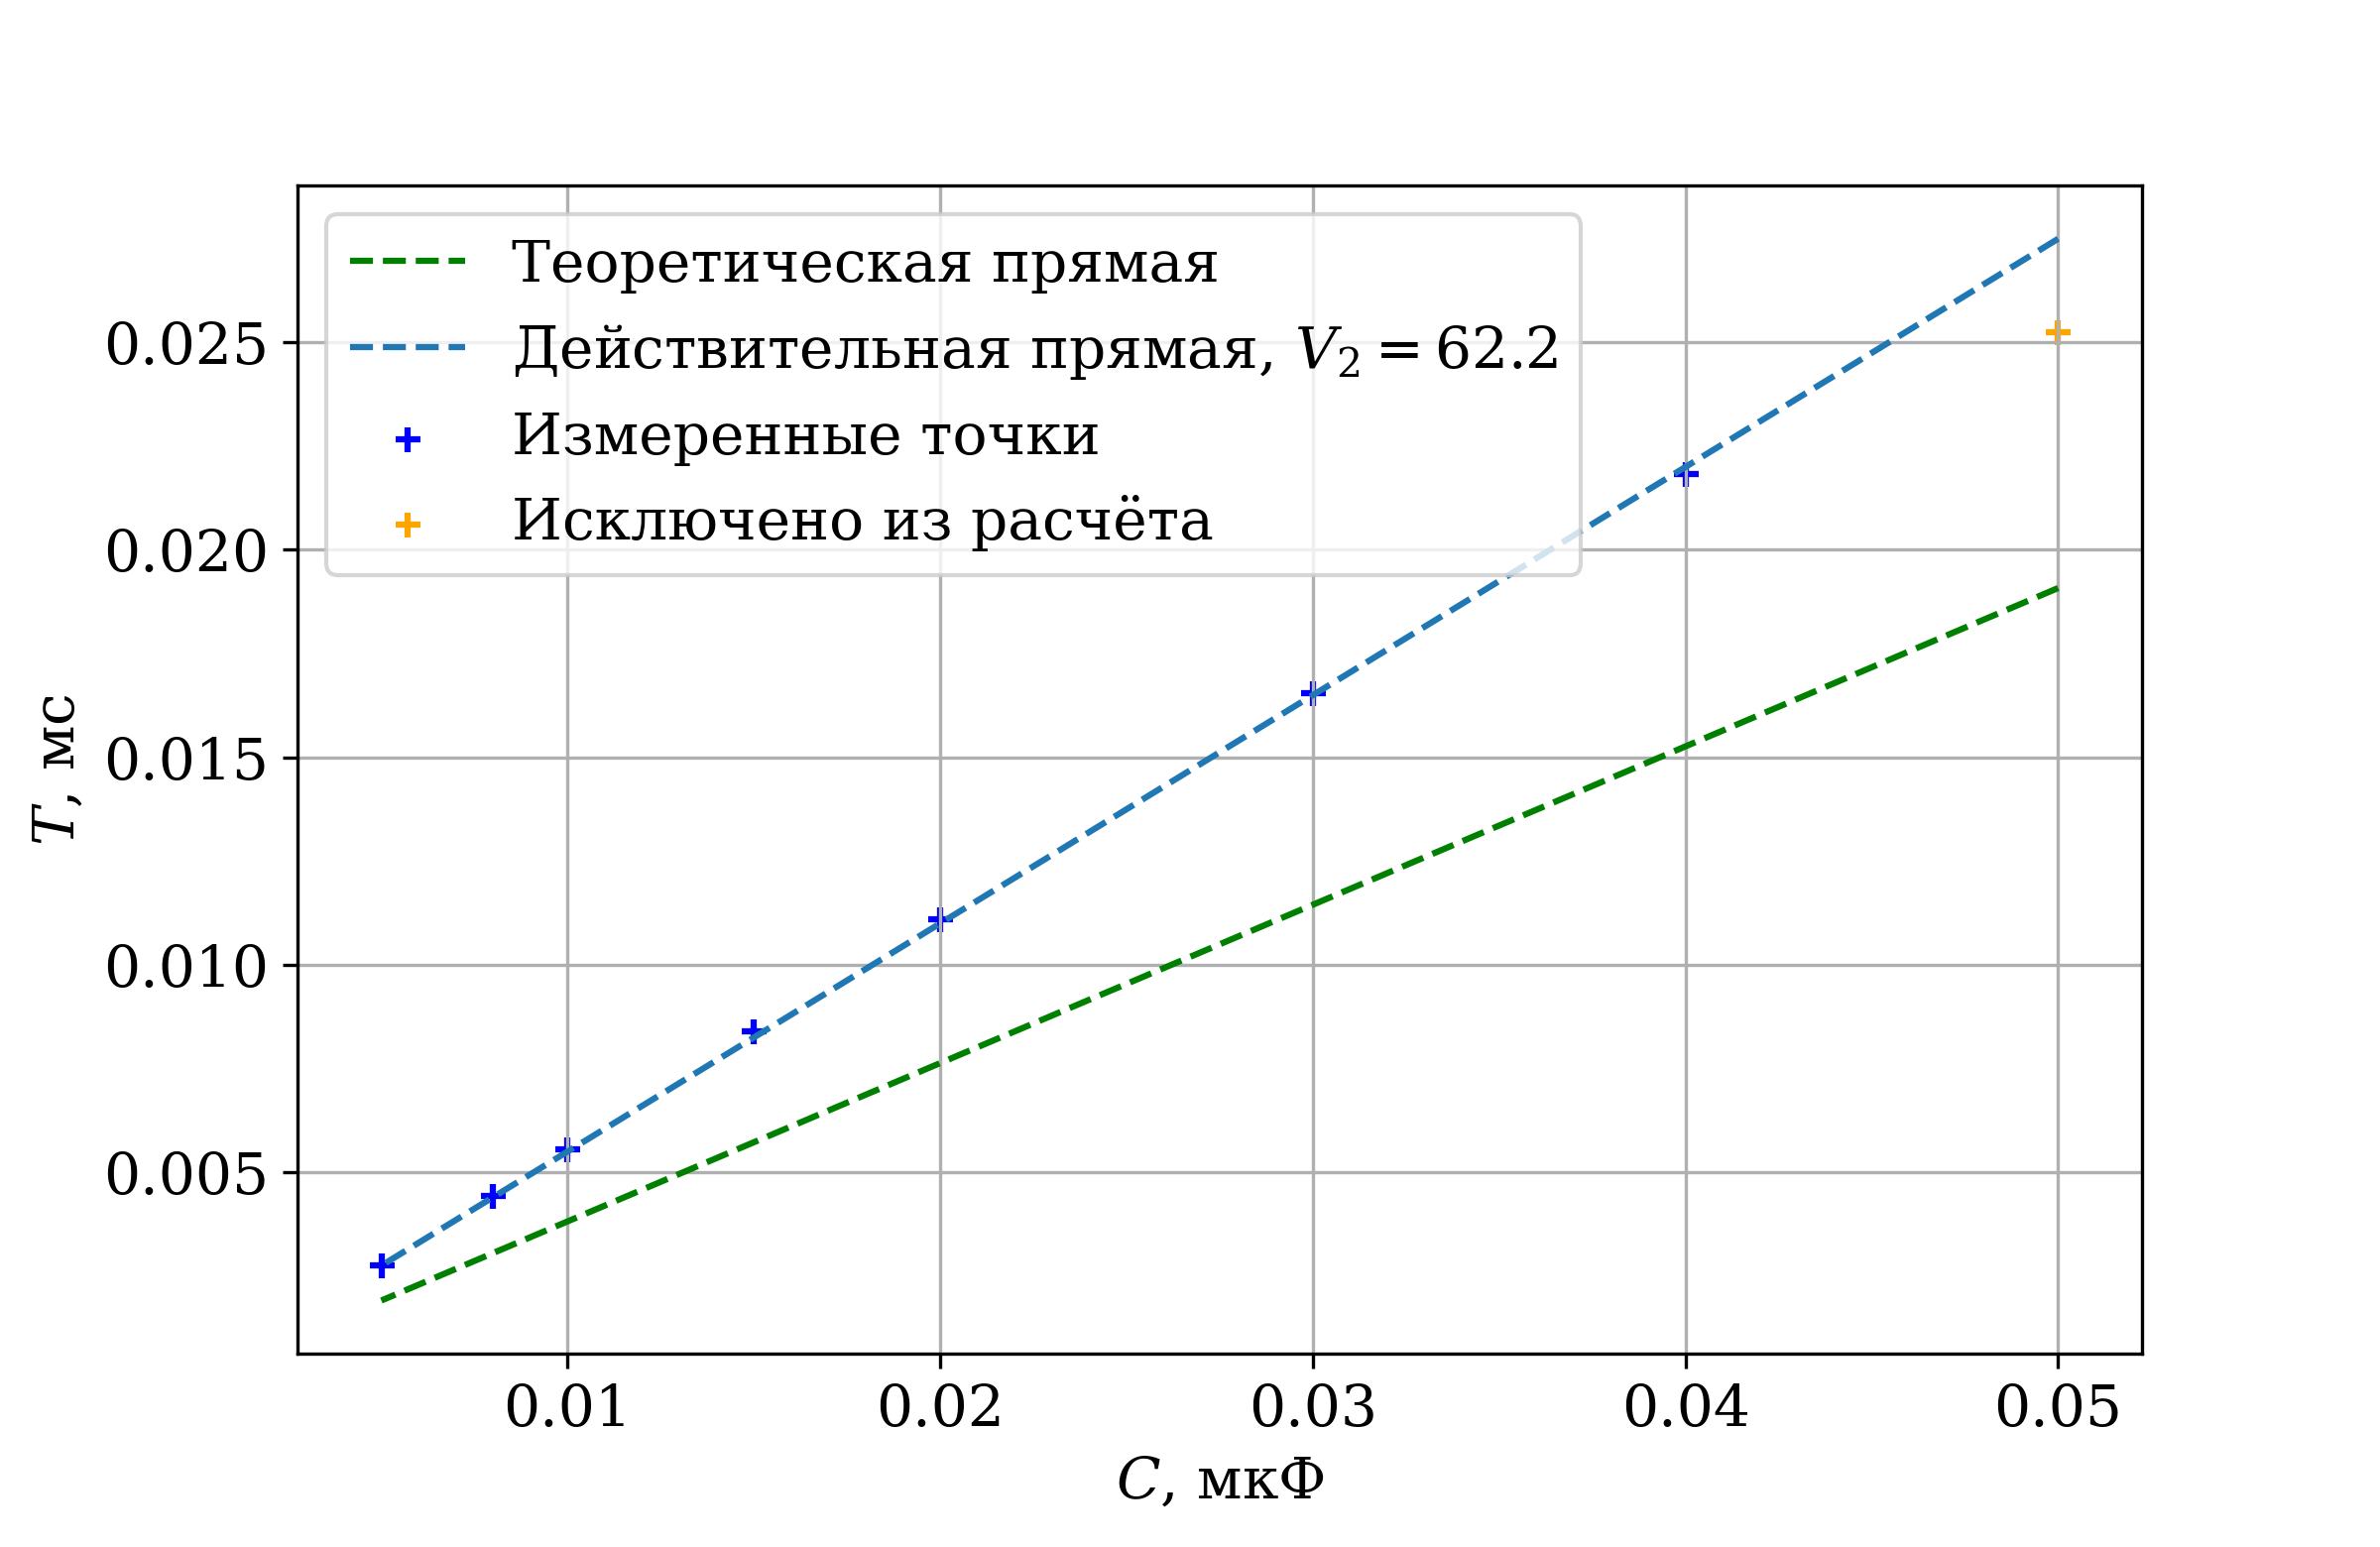
\includegraphics[width=\textwidth]{plot3.png}
\caption{График зависимости $T(C)$}
\label{fig:plot3}
\end{center}
\end{figure}

\begin{figure}
\begin{center}
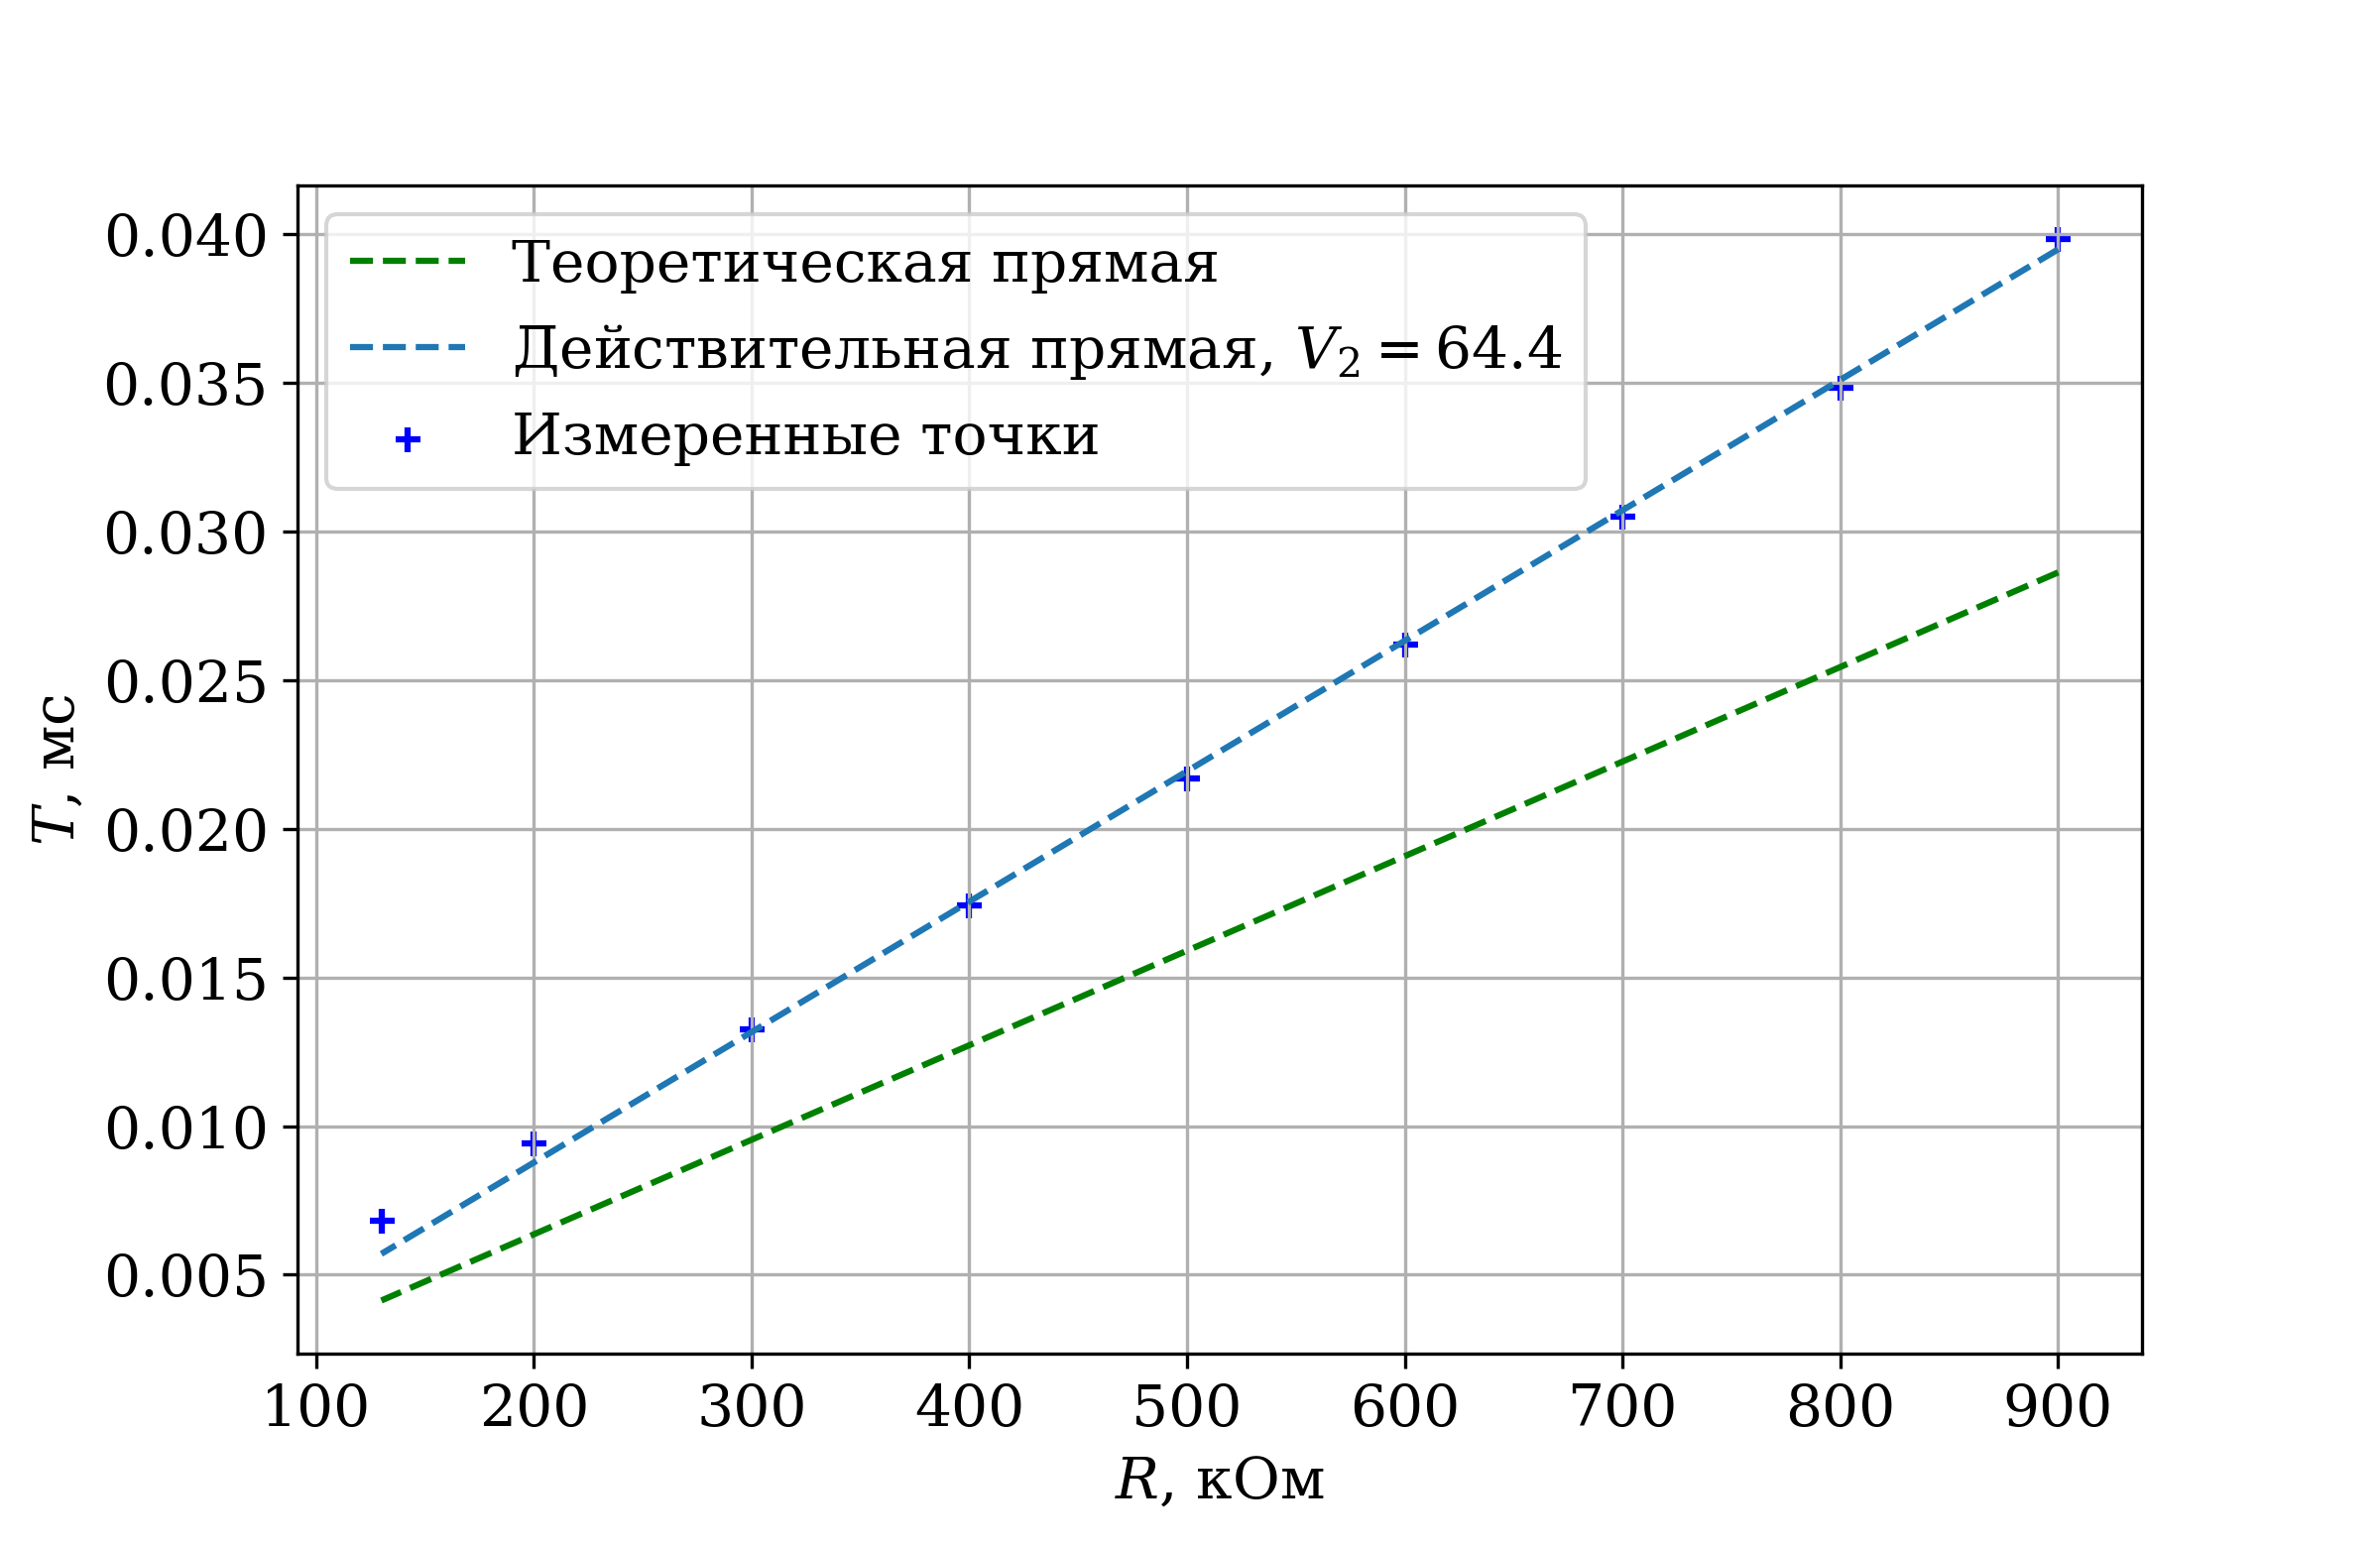
\includegraphics[width=\textwidth]{plot4.png}
\caption{График зависимости $T(R)$}
\label{fig:plot4}
\end{center}
\end{figure}


\medskip\hrule\medskip

\section{Выводы}

Мы изучили нелинейную характеристику стабилитрона, сняв потенциалы зажигания и потухания, и показав, что между ними существует линейный участок.


МЫ показали, что в схеме с конденсатором происходят релаксационные колебания, причём $V_2$ в них отличается от ранее измеренного. 

Получили изображение пилообразных колебаний,и фигур Лиссажу для них, показав возможную схему для получения генератора развёртки на осциллографе.

Так же мы сняли зависимости периода $T(C)$ и $T(R)$, на основе чего почитали значения для $V_2$.

\medskip\hrule\medskip

\end{document}
